
\section{Pengertian Flask}
<<<<<<< HEAD
Flask merupakan sebuah microweb framework yang dicantumkan ke dalam bahasa pemrograman Python berdasar dari Werkzeug toolkit dan template engine Jinja2. Berlisensi BSD. Flask disebut micro framework karena tidak membutuhkan alat-alat tertentu atau pustaka. Flask tidak memiliki database abstraction layer, validasi form, atau komponen lain karena ada pustaka pihak ketiga yang menyediakan fungsi umum.
=======
Flask merupakan sebuah Microweb framework yang dicantumkan ke dalam bahasa pemrograman Python berdasar dari Werkzeug toolkit dan template engine Jinja2. Berlisensi BSD. Flask disebut micro framework karena tidak membutuhkan alat-alat tertentu atau pustaka. Flask tidak memiliki database abstraction layer, validasi form, atau komponen lain karena ada pustaka pihak ketiga yang menyediakan fungsi umum.

\section{Error Handling di Flask}
Error handling dalam flask akan munculnya "Internal Server Erro" pesan yang muncul di sesi terminal saat aplikasi dijalankan. Kemudian akan menampilkan  stack trace dari kesalahan yang terjadi. Stack trace sangat berguna untuk mencari error karena memberikan urutan pemanggilan mana yang menyebabkan sebuah error tersebut terjadi. Stack trace akan memperlihatkan bagian mana yang menjadi penyebabnya. Error ini muncul dari SQLAlchemy yang mencoba menulis username baru ke database, tapi database menolak karena kolom username sebelumnya sudah diatur dengan unique=True.

\subsection{Debug Mode}
Halaman error yang muncul sebelumnya cocok dipakai oleh aplikasi yang sudah diunggah ke sebuah production server. Jika ada error, user akan diberitahu dengan sebuah halaman khusus (yang nanti akan kita perbagus), dengan pesan error yang lebih detail disimpan di file log server.
Tapi saat aplikasinya sedang dibuat, kita tentu menginginkan debug mode untuk diaktifkan. Jika Flask aktif dalam mode ini, kita akan mendapatkan pesan error yang sangat membantu yang akan ditampilkan di browser.

\begin{verbatim}
(venv) $ export FLASK_DEBUG=1
\end{verbatim}

Saat aplikasi sedang dibuat, di butuhkan debug mode untuk mengaktifkan. Apabila Flask aktif dalam mode ini,  pesan error akan muncu dan sangat membantu dan akan ditampilkan di browser. Untuk mengaktifkan debug mode, stop dulu aplikasi, lalu atur environment variable. 
Setelah mengatur FLASK DEBUG, restart ulang server. Pesan yang ditampilkan saat memulai server menjadi agak berbeda dibanding sebelumnya:
\begin{verbatim}
(venv) microblog2 $ flask run
 * Serving Flask app "microblog"
 * Forcing debug mode on
 * Running on http://127.0.0.1:5000/ (Press CTRL+C to quit)
 * Restarting with stat
 * Debugger is active!
 * Debugger PIN: 177-562-960
 \end{verbatim}
 
 Membuat aplikasi crash seperti sebelumnya untuk melihat pesan interactive debugger di browser:
 
 \begin{figure}[ht]
\centerline{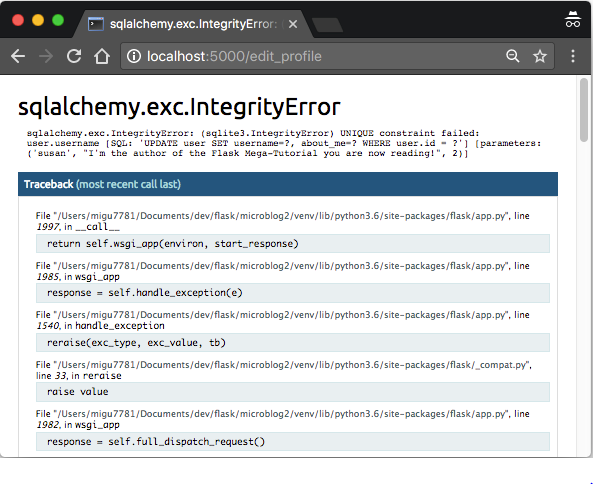
\includegraphics[width=1\textwidth]{figures/5eror.PNG}}
\caption{membuat aplikasi crash.}
\label{eror}
\end{figure}
\ref{eror} dijelaskan bahwa Debugger akan memungkinkan kita meng-expand setiap stack frame dan melihat source code yang terkait. Bisa juga membuka prompt Python di frame manapun dan mengeksekusi perintah Python yang valid, misalnya untuk memeriksa isi dari suatu variabel. Sangat penting untuk tidak mengaktifkan debug mode di production server. Sebagai keamanan tambahan, debugger yang berjalan di browser akan dikunci terlebih dahulu dan meminta nomor PIN yang bisa dilihat saat menjalankan perintah flask run. 


\subsection{Custom Error Pages}
Flask memberikan sebuah mekanisme bagi semua aplikasi untuk memasang halaman error khusus sehingga para user tidak perlu melihat halaman awal yang biasa-biasa saja. Untuk contoh, buat suatu halaman error untuk kode HTTP 404 dan 500, dua kesalahan yang paling sering terjadi pada aplikasi. Membuat halaman untuk halaman error lain tidak berbeda.

Untuk membuat custom error handler, dekorator @errorhandler akan dipakai. Disini akan menulis error handler di file app/errors.py.
app/errors.py: Custom error handlers berikut contohnya :
\begin{verbatim}
from flask import render_template
from app import app, db

@app.errorhandler(404)
def not_found_error(error):
    return render_template('404.html'), 404

@app.errorhandler(500)
def internal_error(error):
    db.session.rollback()
    return render_template('500.html'), 500
 \end{verbatim}
 
Fungsi untuk error handling sangat mirip dengan fungsi view. Untuk kedua jenis error tadi, kita akan menampilkan template khusus. Perhatikan bahwa kedua fungsi tersebut mengirimkan nilai kedua selain template yaitu kode nomor error-nya. Untuk semua fungsi view yang sudah dibuat, tidak perlu mengirimkan kode nomor 200 (untuk menandakan successful response) karena sudah diberikan secara otomatis.
Karena kedua fungsi di atas merupakan fungsi untuk menangani halaman error khusus, maka  perlu memberikan kode status untuk merefleksikan jenis error apa yang akan mereka tangani.

Error handler untuk kode 500 dapat dipanggil setelah sebuah database error, yang salah satu kasusnya terjdi bila ada username yang sama. Untuk memastikan semua percobaan database yang gagal tidak mempengaruhi database yang sudah ada, kita memanggil sesi rollback. Sesi ini akan membersihkan database dari percobaan mengisi data yang sebelumnya gagal (sehingga data yang terubah tidak setengah-setengah).

Berikut ini template untuk halaman error 404:
\begin{verbatim}



    <h1>File Not Found</h1>
    <p><a href="{{ url_for('index') }}">Back</a></p>

 \end{verbatim}
Template meng-extends base.html, sehingga mereka akan memiliki tampilan seperti halaman aplikasi yang normal. 
Agar error handler yang sudah kita tulis terdaftar di Flask, kita perlu mengimpor file app/errors.py sesudah menginisiasi aplikasi
Jika sudah mematikan debug mode dengan FLASK DEBUG 0 di sesi terminal lalu mencoba menganti username sekali lagi, maka kita akan mendapatkan halaman error yang sedikit lebih bersahabat.


\subsection{Mengirim Error Melalui Email}
Masalah lain dengan error handler bawaan Flask adalah tidak ada notifikasi, stack trace untuk setiap error dicetak di terminal, yang artinya output dari proses server harus dimonitor untuk melihat jika terjadi error. Saat aplikasi dijalankan saat melakukan pengembangan hal ini bisa dimaklumi, tapi jika aplikasi sudah di kirim ke server, siapa yang akan memeriksa output yang dikeluarkan? Jadi solusi yang lebih baik diperlukan disini.

Langkah pertama yang mesti dilakukan adalah memberikan detail server email ke file configuration:
Solusi yang akan dilakukan untuk mengatur Flask agar mengirim email setiap terjadi error.
\begin{verbatim}
config.py: Email configuration

class Config(object):
    # ...
    MAIL_SERVER = os.environ.get('MAIL_SERVER')
    MAIL_PORT = int(os.environ.get('MAIL_PORT') or 25)
    MAIL_USE_TLS = os.environ.get('MAIL_USE_TLS') is not None
    MAIL_USERNAME = os.environ.get('MAIL_USERNAME')
    MAIL_PASSWORD = os.environ.get('MAIL_PASSWORD')
    ADMINS = ['your-email@example.com']
    \end{verbatim} 
    
Variabel configuration untuk email diantaranya adalah server, port, penanda untuk mengaktifkan koneksi terenkripsi atau tidak, disertai dengan username dan password. Kelima variabel diambil dari environment variable. Jika server email tidak diatur di environment variable, maka itu akan menjadi pertanda bahwa pengiriman error email perlu dimatikan. Port server email juga perlu dimasukkan di environment variable, tapi jika tidak diatur, port standar nomor 25 akan dipakai. Data username dan password tidak wajib diberikan. Variabel ADMIN adalah daftar email yang akan menerima email error.

Flask menggunakan paket logging dari Python untuk menulis log dan  sudah memiliki kemampuan untuk mengirim log via email. Yang perlu dilakukan untuk mengirimkan pesan log tersebut ke email adalah menambahkan sebuah instance SMTPHandler ke objek Flask logger, yang bernama app.logger  kita hanya akan mengaktifkan email logger jika aplikasi dijalankan tanpa debug mode saat nilai app.debug berisi True juga saat server email ada di file configuration.

Kode-kode di atas akan membuat sebuah instance dari SMTPHandler, mengatur level-nya sehingga hanya membuat laporan error bukan warning, informational atau debugging message, lalu mengirim laporan error tersebut ke objek app.logger dari Flask. Ada dua cara untuk menguji fitur ini. Cara pailng mudah ialah dengan menggunakan server debugging SMTP dari Python. Server ini adalah server email fake , bukannya mengirim, ia akan mencetak email ke console (terminal). 

Untuk menguji kode yang kita buat dengan server ini, atur MAIL_SERVER=localhost dan MAIL_PORT=8025. Jika menggunakan Linux atau Mac OS, perlu menggunakan perintah sudo sehingga perintah tersebut bisa dijalankan. Jika menggunakan Windows, pastikan membuka aplikasi cmd sebagai administrator. Hak akses admin diperlukan dikarenakan port di bawah dari 1024 adalah port yang hanya bisa dijalankan oleh administrator. 

Biarkan server SMTP berjalan lalu kembali ke terminal awal, jalankan perintah export. MAIL_SERVER=localhost dan MAIL_PORT=8025. Pastikan variabel FLASK_DEBUG sudah diatur menjadi 0 atau tidak diatur sama sekali, sehingga aplikasi tidak mengirim email dalam debug mode. Jalankan aplikasi dan picu error. SQLAlchemy digunakan untuk melihat terminal yang menjalankan server email fake  yang akan menampilkan sebuah pesan email dengan kode-kode error.
